\documentclass[bigtut]{tutorial}\usepackage[]{graphicx}\usepackage[]{color}
%% maxwidth is the original width if it is less than linewidth
%% otherwise use linewidth (to make sure the graphics do not exceed the margin)
\makeatletter
\def\maxwidth{ %
  \ifdim\Gin@nat@width>\linewidth
    \linewidth
  \else
    \Gin@nat@width
  \fi
}
\makeatother

\definecolor{fgcolor}{rgb}{0.345, 0.345, 0.345}
\newcommand{\hlnum}[1]{\textcolor[rgb]{0.686,0.059,0.569}{#1}}%
\newcommand{\hlstr}[1]{\textcolor[rgb]{0.192,0.494,0.8}{#1}}%
\newcommand{\hlcom}[1]{\textcolor[rgb]{0.678,0.584,0.686}{\textit{#1}}}%
\newcommand{\hlopt}[1]{\textcolor[rgb]{0,0,0}{#1}}%
\newcommand{\hlstd}[1]{\textcolor[rgb]{0.345,0.345,0.345}{#1}}%
\newcommand{\hlkwa}[1]{\textcolor[rgb]{0.161,0.373,0.58}{\textbf{#1}}}%
\newcommand{\hlkwb}[1]{\textcolor[rgb]{0.69,0.353,0.396}{#1}}%
\newcommand{\hlkwc}[1]{\textcolor[rgb]{0.333,0.667,0.333}{#1}}%
\newcommand{\hlkwd}[1]{\textcolor[rgb]{0.737,0.353,0.396}{\textbf{#1}}}%

\usepackage{framed}
\makeatletter
\newenvironment{kframe}{%
 \def\at@end@of@kframe{}%
 \ifinner\ifhmode%
  \def\at@end@of@kframe{\end{minipage}}%
  \begin{minipage}{\columnwidth}%
 \fi\fi%
 \def\FrameCommand##1{\hskip\@totalleftmargin \hskip-\fboxsep
 \colorbox{shadecolor}{##1}\hskip-\fboxsep
     % There is no \\@totalrightmargin, so:
     \hskip-\linewidth \hskip-\@totalleftmargin \hskip\columnwidth}%
 \MakeFramed {\advance\hsize-\width
   \@totalleftmargin\z@ \linewidth\hsize
   \@setminipage}}%
 {\par\unskip\endMakeFramed%
 \at@end@of@kframe}
\makeatother

\definecolor{shadecolor}{rgb}{.97, .97, .97}
\definecolor{messagecolor}{rgb}{0, 0, 0}
\definecolor{warningcolor}{rgb}{1, 0, 1}
\definecolor{errorcolor}{rgb}{1, 0, 0}
\newenvironment{knitrout}{}{} % an empty environment to be redefined in TeX

\usepackage{alltt}
\unitcode{MATH1005}
        \unitname{Statistics}
        \semester{Summer/Winter/Semester2}
        \sheetnumber6

\usepackage{graphicx}
\usepackage{tikz}
\withsolutions
\IfFileExists{upquote.sty}{\usepackage{upquote}}{}
\begin{document}
\lettersfirst

\begin{tutorial}

\begin{center}
\begin{tabular}{| ll |} \hline
& \\
{\bf Discrete Random Variables} & \\
For a discrete random variable $X$ & \\
probability distribution &   $ \{ x, P(X=x) \}$  \hspace{.2cm} (often represented in table)    \\
expected value or mean & $E(X) = \sum_{x}^{} x P(X=x)$      \\ 
expected value of function  & $E(f(X)) = \sum_{x}^{} f(x) P(X=x)$    \\
  & Eg: $E(X^2) = \sum_{x}^{} x^2 P(X=x)$    \\
variance & $ Var(X) = E(X^2) - E(X)^2 $ \\ 
& \\  \hline
\end{tabular}
\end{center}

\begin{center}
\fbox{
\begin{minipage}{6in}  
\vspace{.5cm}
{\bf Combinatorial coefficients}  \\  \\
${N \choose n} = \frac{N!}{n! (N-n)!}$    \hspace{.5cm} where $N! = N(N-1)(N-2) \ldots 1$ \\ \\
\end{minipage}
}
\end{center}


\begin{center}
\fbox{
\begin{minipage}{6in} 
\vspace{.5cm}
{\bf Eg1: Generalised Hypergeometric Distribution (Sampling without replacement)}  \\
Given an urn of size $N$ with $N_1$ balls of  type 1, $N_2$ balls of  type 2, ... $N_k$ balls of  type $k$.  \\
Draw a sample of size $n$ without replacement. \\
\[ P(\mbox{Select $n_i$ balls of each type $i$ })  =\frac{ {N_1 \choose n_1}   {N_2 \choose n_2} \ldots {N_k \choose n_k}}{{N \choose n}} \] 
\vspace{.3cm}
\end{minipage}
}
\end{center}

\begin{center}
\fbox{
\begin{minipage}{5.5in}
\vspace{.5cm}
{\bf Eg2: Binomial Distribution (Sampling with replacement)}  \\ 
Consider a sequence of $n$ independent, Binary trials with probability of success $p$, and let $X$ count the number of successes. 

\[  P(X=x) = {n \choose x} p^x (1-p)^{n-x}  \hspace{.5cm} \text{for } x=0,1,\ldots,n  \]

\vspace{.3cm}
Moments: $E(X) = np$, $Var(X)=np(1-p)$

\end{minipage}
}
\end{center}

\newpage
\begin{questions}
\question Combinatorial coefficients \\

\begin{parts}
\part By hand, show that $6! = 720$, ${6 \choose 0} = 1$ and ${6 \choose 3} = 20$. 

\part Confirm your answers by finding the correct button on your calculator, and by using R:

\begin{knitrout}
\definecolor{shadecolor}{rgb}{0.969, 0.969, 0.969}\color{fgcolor}\begin{kframe}
\begin{alltt}
\hlkwd{factorial}\hlstd{(}\hlnum{6}\hlstd{)}
\hlkwd{choose}\hlstd{(}\hlnum{6}\hlstd{,}\hlnum{0}\hlstd{)}
\end{alltt}
\end{kframe}
\end{knitrout}

\part What does ${6 \choose x}$ represent?
\end{parts}

\begin{solution}
(c) ${6 \choose x}$ represents the number of ways of choosing $x$ items from 6, where $x=0,1,2,3,4,5,6$.
\end{solution}


\question Modelling M\&Ms \\

\begin{parts}
\item According to the following article, what are the proportions of colours of M\&Ms in each standard pack?
{\tiny http://joshmadison.com/mms-color-distribution-analysis/}


\vspace{.5cm}
\begin{center}
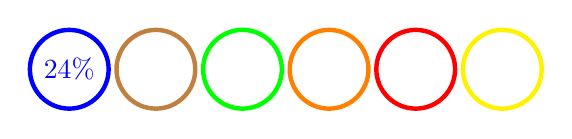
\begin{tikzpicture}
\draw [blue, fill=white, ultra thick] (-0.3,1.5) circle [radius=0.5] node {24\%};;
\draw [brown, fill=white, ultra thick] (0.8,1.5) circle [radius=0.5] node {};;
\draw [green, fill=white, ultra thick] (1.9,1.5) circle [radius=0.5] node {};;
\draw [orange, fill=white, ultra thick] (3,1.5) circle [radius=0.5] node {};;
\draw [red, fill=white, ultra thick] (4.1,1.5) circle [radius=0.5] node {};;
\draw [yellow, fill=white, ultra thick] (5.2,1.5) circle [radius=0.5] node {};;
\end{tikzpicture}
\end{center}


\vspace{.5cm}
\item 
If I randomly pick 10 M\&Ms from a certain packet containing 100 M\&Ms, what is the chance that I get 2 blues.

\vspace{.5cm}
\begin{center}
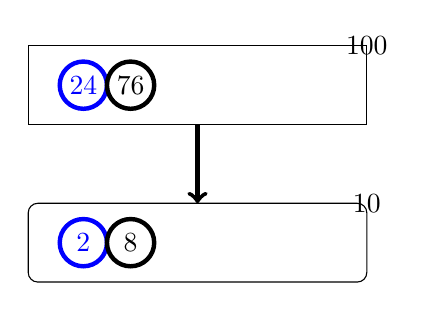
\begin{tikzpicture}
\draw [black] (-1,1) rectangle (3.3,2) node {100};
\draw [blue, fill=white, ultra thick] (-0.3,1.5) circle [radius=0.3] node {24};;
\draw [black, fill=white, ultra thick] (0.3,1.5) circle [radius=0.3] node {76};;

\draw [->, black, ultra thick]  (1.15,1) -- (1.15,0);

\draw [black, rounded corners=.8ex] (-1,-1) rectangle (3.3,0) node {10};
\draw [blue, fill=white, ultra thick] (-0.3,-0.5) circle [radius=0.3] node {2};;
\draw [black, fill=white, ultra thick] (0.3,-0.5) circle [radius=0.3] node {8};;
\end{tikzpicture}
\end{center}

\vspace{.5cm}
\item 
If I randomly pick 6 M\&Ms from a certain packet containing 100 M\&Ms, what is the chance that I get 1 of each colour?

\vspace{.5cm}
\begin{center}
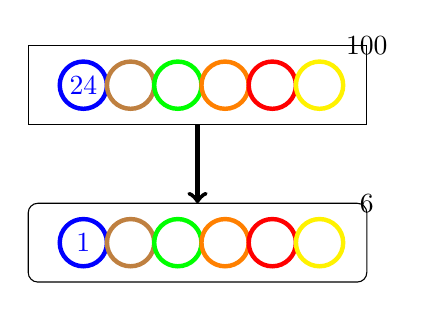
\begin{tikzpicture}
\draw [black] (-1,1) rectangle (3.3,2) node {100};
\draw [blue, fill=white, ultra thick] (-0.3,1.5) circle [radius=0.3] node {24};;
\draw [brown, fill=white, ultra thick] (0.3,1.5) circle [radius=0.3] node {};;
\draw [green, fill=white, ultra thick] (0.9,1.5) circle [radius=0.3] node {};;
\draw [orange, fill=white, ultra thick] (1.5,1.5) circle [radius=0.3] node {};;
\draw [red, fill=white, ultra thick] (2.1,1.5) circle [radius=0.3] node {};;
\draw [yellow, fill=white, ultra thick] (2.7,1.5) circle [radius=0.3] node {};;

\draw [->, black, ultra thick]  (1.15,1) -- (1.15,0);

\draw [black, rounded corners=.8ex] (-1,-1) rectangle (3.3,0) node {6};
\draw [blue, fill=white, ultra thick] (-0.3,-0.5) circle [radius=0.3] node {1};;
\draw [brown, fill=white, ultra thick] (0.3,-0.5) circle [radius=0.3] node {};;
\draw [green, fill=white, ultra thick] (0.9,-0.5) circle [radius=0.3] node {};;
\draw [orange, fill=white, ultra thick] (1.5,-0.5) circle [radius=0.3] node {};;
\draw [red, fill=white, ultra thick] (2.1,-0.5) circle [radius=0.3] node {};;
\draw [yellow, fill=white, ultra thick] (2.7,-0.5) circle [radius=0.3] node {};;
\end{tikzpicture}
\end{center}




\vspace{.5cm}
\item 
M\&Ms runs a competition with a gift voucher in 10\% of packets. Suppose I buy 20 packets. What is the chance that I don't get any vouchers.
\end{parts}


\begin{solution}

\begin{parts}

\item
Blue: 24\%, Brown 14\%, Green 16\%, Orange 20\%, Red 13\%, Yellow 14\%.

\item
Model the packet by a hypergeometric. \\
$N=100$, $N_{1} = \mbox{Number of Blues} = 24$ and $N_{2} = \mbox{Number of non-blues} = 76$; $n=10$.

\vspace{.5cm}
\begin{center}
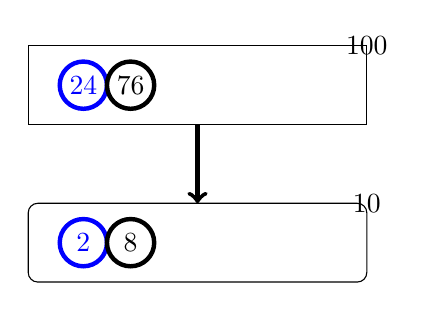
\begin{tikzpicture}
\draw [black] (-1,1) rectangle (3.3,2) node {100};
\draw [blue, fill=white, ultra thick] (-0.3,1.5) circle [radius=0.3] node {24};;
\draw [black, fill=white, ultra thick] (0.3,1.5) circle [radius=0.3] node {76};;

\draw [->, black, ultra thick]  (1.15,1) -- (1.15,0);

\draw [black, rounded corners=.8ex] (-1,-1) rectangle (3.3,0) node {10};
\draw [blue, fill=white, ultra thick] (-0.3,-0.5) circle [radius=0.3] node {2};;
\draw [black, fill=white, ultra thick] (0.3,-0.5) circle [radius=0.3] node {8};;
\end{tikzpicture}
\end{center}


$P(\mbox{2 blue, 8 non-blues}) = \frac{{24 \choose 2}{76 \choose 8}}{{100 \choose 10}} \approx 0.3$.

\begin{knitrout}
\definecolor{shadecolor}{rgb}{0.969, 0.969, 0.969}\color{fgcolor}\begin{kframe}
\begin{alltt}
\hlkwd{choose}\hlstd{(}\hlnum{24}\hlstd{,}\hlnum{2}\hlstd{)}\hlopt{*}\hlkwd{choose}\hlstd{(}\hlnum{76}\hlstd{,}\hlnum{8}\hlstd{)}\hlopt{/}\hlkwd{choose}\hlstd{(}\hlnum{100}\hlstd{,}\hlnum{10}\hlstd{)}
\end{alltt}
\begin{verbatim}
## [1] 0.300643
\end{verbatim}
\begin{alltt}
\hlkwd{dhyper}\hlstd{(}\hlnum{2}\hlstd{,}\hlnum{24}\hlstd{,}\hlnum{76}\hlstd{,}\hlnum{10}\hlstd{,}\hlkwc{log}\hlstd{=}\hlnum{FALSE}\hlstd{)}
\end{alltt}
\begin{verbatim}
## [1] 0.300643
\end{verbatim}
\end{kframe}
\end{knitrout}


\item
Model the packet by a hypergeometric. \\
$N=100$, $N_{1} = \mbox{Number of Blues} = 24$; $N_{2} = \mbox{Number of Browns} = 14$, $\ldots$, $N_{6} = \mbox{Number of Yellows} = 14$; $n=6$.


\vspace{.5cm}
\begin{center}
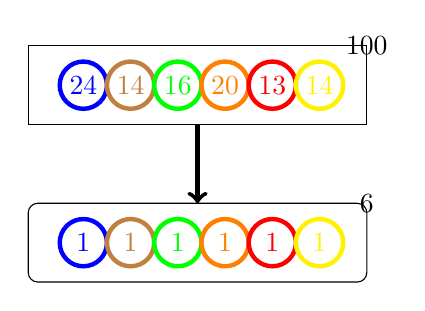
\begin{tikzpicture}
\draw [black] (-1,1) rectangle (3.3,2) node {100};
\draw [blue, fill=white, ultra thick] (-0.3,1.5) circle [radius=0.3] node {24};;
\draw [brown, fill=white, ultra thick] (0.3,1.5) circle [radius=0.3] node {14};;
\draw [green, fill=white, ultra thick] (0.9,1.5) circle [radius=0.3] node {16};;
\draw [orange, fill=white, ultra thick] (1.5,1.5) circle [radius=0.3] node {20};;
\draw [red, fill=white, ultra thick] (2.1,1.5) circle [radius=0.3] node {13};;
\draw [yellow, fill=white, ultra thick] (2.7,1.5) circle [radius=0.3] node {14};;

\draw [->, black, ultra thick]  (1.15,1) -- (1.15,0);

\draw [black, rounded corners=.8ex] (-1,-1) rectangle (3.3,0) node {6};
\draw [blue, fill=white, ultra thick] (-0.3,-0.5) circle [radius=0.3] node {1};;
\draw [brown, fill=white, ultra thick] (0.3,-0.5) circle [radius=0.3] node {1};;
\draw [green, fill=white, ultra thick] (0.9,-0.5) circle [radius=0.3] node {1};;
\draw [orange, fill=white, ultra thick] (1.5,-0.5) circle [radius=0.3] node {1};;
\draw [red, fill=white, ultra thick] (2.1,-0.5) circle [radius=0.3] node {1};;
\draw [yellow, fill=white, ultra thick] (2.7,-0.5) circle [radius=0.3] node {1};;
\end{tikzpicture}
\end{center}


$P(\mbox{1 of each colour}) = \frac{{24 \choose 1}{14 \choose 1}{16 \choose 1}{20 \choose 1}{13\choose 1}{14 \choose 1}}{{100 \choose 6}} \approx 0.02$.

{\tiny
\begin{knitrout}
\definecolor{shadecolor}{rgb}{0.969, 0.969, 0.969}\color{fgcolor}\begin{kframe}
\begin{alltt}
\hlkwd{choose}\hlstd{(}\hlnum{24}\hlstd{,}\hlnum{1}\hlstd{)}\hlopt{*}\hlkwd{choose}\hlstd{(}\hlnum{14}\hlstd{,}\hlnum{1}\hlstd{)}\hlopt{*}\hlkwd{choose}\hlstd{(}\hlnum{16}\hlstd{,}\hlnum{1}\hlstd{)}\hlopt{*}\hlkwd{choose}\hlstd{(}\hlnum{20}\hlstd{,}\hlnum{1}\hlstd{)}\hlopt{*}\hlkwd{choose}\hlstd{(}\hlnum{13}\hlstd{,}\hlnum{1}\hlstd{)}\hlopt{*}\hlkwd{choose}\hlstd{(}\hlnum{14}\hlstd{,}\hlnum{1}\hlstd{)}\hlopt{/}\hlkwd{choose}\hlstd{(}\hlnum{100}\hlstd{,}\hlnum{6}\hlstd{)}
\end{alltt}
\begin{verbatim}
## [1] 0.01641592
\end{verbatim}
\end{kframe}
\end{knitrout}
}

\item 
Model the competition by a Binomial. \\
$X = \mbox{The total number of vouchers in 20 packets} \sim Bin(n=20,p=0.1)$. \\
$P(X=0) = {20 \choose 0} (0.1)^0 (0.9)^{20} \approx 0.12$.

\begin{knitrout}
\definecolor{shadecolor}{rgb}{0.969, 0.969, 0.969}\color{fgcolor}\begin{kframe}
\begin{alltt}
\hlkwd{choose}\hlstd{(}\hlnum{20}\hlstd{,}\hlnum{0}\hlstd{)}\hlopt{*}\hlstd{(}\hlnum{0.1}\hlopt{^}\hlnum{0}\hlstd{)}\hlopt{*}\hlstd{(}\hlnum{0.9}\hlopt{^}\hlnum{20}\hlstd{)}
\end{alltt}
\begin{verbatim}
## [1] 0.1215767
\end{verbatim}
\begin{alltt}
\hlkwd{dbinom}\hlstd{(}\hlnum{0}\hlstd{,}\hlnum{20}\hlstd{,}\hlnum{0.1}\hlstd{)}
\end{alltt}
\begin{verbatim}
## [1] 0.1215767
\end{verbatim}
\end{kframe}
\end{knitrout}

\end{parts}

Note: Any data drawn from a blog must be scrutinised in terms of reliability. A more reliable source of information about M\&Ms is found here: \\
http://www.maths.usyd.edu.au/u/UG/JM/MATH1005/r/loc/Mars.pdf
\end{solution}

\newpage
\question Simulating a Binomial Distribution \\

\begin{parts}
\part  Suppose that $X \sim B(4, 0.2)$. State the mean, variance and standard deviation of $X$.

\vspace{.5cm}
\part Using the Binomial distribution formula, complete the following table

\begin{center}
\begin{tabular}{| l | l | l | l | l | l | l|} \hline
x & 0  \hspace{1cm} & 1 \hspace{1cm}  & 2 \hspace{1cm} & 3 \hspace{1cm} & 4 \hspace{1cm}  &  Total \\ \hline
$P(X=x)$ & 0.4096 & & &  & 0.0016  & 1  \\ \hline
\end{tabular}
\end{center}

\vspace{.5cm}
\part Using the table, calculate $E(X)$, $E(X^2)$ and $Var(X)$.
Check that this agrees with (a).

\begin{knitrout}
\definecolor{shadecolor}{rgb}{0.969, 0.969, 0.969}\color{fgcolor}\begin{kframe}
\begin{alltt}
\hlcom{#Check answers in R}
\hlstd{x}\hlkwb{=}\hlkwd{c}\hlstd{(}\hlnum{0}\hlopt{:}\hlnum{4}\hlstd{)}
\hlstd{p}\hlkwb{=}\hlkwd{dbinom}\hlstd{(x,}\hlnum{4}\hlstd{,}\hlnum{0.2}\hlstd{)}
\hlkwd{sum}\hlstd{(x}\hlopt{*}\hlstd{p)}
\hlkwd{sum}\hlstd{(x}\hlopt{^}\hlnum{2}\hlopt{*}\hlstd{p)}
\hlkwd{sum}\hlstd{(x}\hlopt{^}\hlnum{2}\hlopt{*}\hlstd{p)}\hlopt{-}\hlkwd{sum}\hlstd{(x}\hlopt{*}\hlstd{p)}\hlopt{^}\hlnum{2}
\end{alltt}
\end{kframe}
\end{knitrout}

\vspace{.5cm}
\part Using the table, find $P (X \leq 3)$.  Check you can also get this answer from the Binomial tables and by using R.
\begin{knitrout}
\definecolor{shadecolor}{rgb}{0.969, 0.969, 0.969}\color{fgcolor}\begin{kframe}
\begin{alltt}
\hlkwd{pbinom}\hlstd{(}\hlnum{3}\hlstd{,}\hlnum{4}\hlstd{,}\hlnum{0.2}\hlstd{)}
\end{alltt}
\begin{verbatim}
## [1] 0.9984
\end{verbatim}
\end{kframe}
\end{knitrout}

\vspace{.5cm}
\part
Simulate the distribution by generating 100 random variables from $X \sim Bin(n=4, p=0.2)$.

\begin{knitrout}
\definecolor{shadecolor}{rgb}{0.969, 0.969, 0.969}\color{fgcolor}\begin{kframe}
\begin{alltt}
\hlkwd{set.seed}\hlstd{(}\hlnum{1234}\hlstd{)}       \hlcom{#Chooses the random number generator}
\hlstd{x}\hlkwb{=}\hlkwd{rbinom}\hlstd{(}\hlnum{100}\hlstd{,}\hlnum{4}\hlstd{,}\hlnum{0.2}\hlstd{)}  \hlcom{#Simulates 100 numbers from a Bin(4,0.2)}
\hlkwd{plot}\hlstd{(}\hlkwd{table}\hlstd{(x))}       \hlcom{#Produces a frequency table of simulations}
\hlkwd{hist}\hlstd{(x)}              \hlcom{#Produces a histogram of simulations}
\hlkwd{mean}\hlstd{(x)}              \hlcom{#Produces mean of simulations}
\hlkwd{var}\hlstd{(x)}               \hlcom{#Produces the variance of simulations}
\end{alltt}
\end{kframe}
\end{knitrout}
\end{parts}

\begin{solution}
(a) 
Given $X \sim B(4, 0.2)$, \\
$E(X) = np = 4 \times 0.2 = 0.8$. \\
$Var(X) = np(1-p) = 4 \times 0.2 \times 0.8 = 0.64$. \\
$SD(X) = \sqrt{0.64} = 0.8$.

\vspace{.5cm}
(b) \\
\begin{tabular}{| l | l | l | l | l | l | l|} \hline
x & 0  \hspace{1cm} & 1 \hspace{1cm}  & 2 \hspace{1cm} & 3 \hspace{1cm} & 4 \hspace{1cm}  &  Total \\ \hline
$P(X=x)$ & 0.4096  & 0.4096 & 0.1536 & 0.0256 & 0.0016 & 1 \\ \hline
\end{tabular}

\vspace{.5cm}
Working: \\
$P(X=0) = {4 \choose 0} (0.2)^0 (0.8)^4 = 0.4096 $ \\
$P(X=1) = {4 \choose 1} (0.2)^1 (0.8)^3 = 0.4096 $ \\
$P(X=2) = {4 \choose 2} (0.2)^2 (0.8)^2 = 0.1536 $ \\
$P(X=3) = {4 \choose 3} (0.2)^3 (0.8)^1 = 0.0256 $ \\
$P(X=4) = {4 \choose 4} (0.2)^4 (0.8)^0 = 0.0016  $\\


\vspace{.5cm}
(c)
$E(X) = 0 \times 0.4096 + 1 \times 0.4096 + 2 \times 
0.1536 + 3 \times 0.0256 + 4 \times 0.0016 = 0.8$ \\
Agrees with (a). \\

$E(X^2) = 0^2 \times 0.4096 + 1^2 \times 0.4096 + 2^2 \times  0.1536 + 3^2 \times 0.0256 + 4^2 \times 0.0016 = 1.28$ \\

$Var(X) = 1.28 - (.8)^2 =0.64$.
Agrees with (a). \\


\vspace{.5cm}
(d)
$P (X \leq 3) = P(0) + P(1) + P(2) + P(3) = 0.9984 $. \\ 
Or $P (X \leq 3) = 1-P(X=4) = 1-0.0016 =0.9984 $.

\begin{knitrout}
\definecolor{shadecolor}{rgb}{0.969, 0.969, 0.969}\color{fgcolor}\begin{kframe}
\begin{alltt}
\hlkwd{pbinom}\hlstd{(}\hlnum{3}\hlstd{,}\hlnum{4}\hlstd{,}\hlnum{0.2}\hlstd{)}
\end{alltt}
\begin{verbatim}
## [1] 0.9984
\end{verbatim}
\end{kframe}
\end{knitrout}
\end{solution}


\newpage
\hspace{-1cm} {\bf Extra Questions}

\question Expected values and variance \\

Given the following probability distribution table

\begin{center}
\begin{tabular}{| l | l | l | l | l | l |} \hline
$x$ & 1 \hspace{1cm}  & 2 \hspace{1cm} & 3 \hspace{1cm} & 4 \hspace{1cm}  &  Total \\ \hline
$P(X=x)$ & 0.1 & 0.2 & 0.3 & 0.4 & 1 \\ \hline
\end{tabular}
\end{center}

\begin{parts}

\part  What is the formula for the probability distribution function?

\part
By hand, find $E(X), E(X^2)$, $E(\frac{1}{X})$ and $Var(X)$? \\

\begin{knitrout}
\definecolor{shadecolor}{rgb}{0.969, 0.969, 0.969}\color{fgcolor}\begin{kframe}
\begin{alltt}
\hlcom{#Check answers in R}
\hlstd{x}\hlkwb{=}\hlkwd{c}\hlstd{(}\hlnum{1}\hlopt{:}\hlnum{4}\hlstd{)}
\hlstd{p}\hlkwb{=}\hlstd{x}\hlopt{/}\hlnum{10}
\hlkwd{sum}\hlstd{(x}\hlopt{*}\hlstd{p)}
\hlkwd{sum}\hlstd{(x}\hlopt{^}\hlnum{2}\hlopt{*}\hlstd{p)}
\hlkwd{sum}\hlstd{((}\hlnum{1}\hlopt{/}\hlstd{x)}\hlopt{*}\hlstd{p)}
\hlkwd{sum}\hlstd{(x}\hlopt{^}\hlnum{2}\hlopt{*}\hlstd{p)} \hlopt{-} \hlkwd{sum}\hlstd{(x}\hlopt{*}\hlstd{p)}\hlopt{^}\hlnum{2}
\end{alltt}
\end{kframe}
\end{knitrout}

\part Estimate your answers by simulation.
\begin{knitrout}
\definecolor{shadecolor}{rgb}{0.969, 0.969, 0.969}\color{fgcolor}\begin{kframe}
\begin{alltt}
\hlstd{y}\hlkwb{=}\hlkwd{sample}\hlstd{(x,} \hlnum{10000}\hlstd{,} \hlkwc{prob}\hlstd{=p,} \hlkwc{replace}\hlstd{=T)}   \hlcom{#Simulates 10000 draws}
\hlkwd{mean}\hlstd{(y)}
\hlkwd{mean}\hlstd{(y}\hlopt{^}\hlnum{2}\hlstd{)}
\hlkwd{mean}\hlstd{(}\hlnum{1}\hlopt{/}\hlstd{y)}
\hlkwd{var}\hlstd{(y)}
\end{alltt}
\end{kframe}
\end{knitrout}
\end{parts}

\begin{solution}
(a) $P(X=x) = \frac{x}{10}$ for $x=1,2,3,4$.\\

(b) 
$E(X) =\sum_{i=1}^{n} x P(X=x) = 1 \times 0.1 + 2 \times 0.2 + 3 \times 0.3 + 4 \times 0.4 = 3$ \\
$E(X^2) =\sum_{i=1}^{n} x^2 P(X=x) = 1^2 \times 0.1 + 2^2 \times 0.2 + 3^2 \times 0.3 + 4^2 \times 0.4 = 10$ \\
$E(1/X) =\sum_{i=1}^{n} 1/x P(X=x) = 1/1 \times 0.1 + 1/2 \times 0.2 + 1/3 \times 0.3 + 1/4 \times 0.4 = 0.4$ \\
$Var(X) = E(X^2) - E^2(X) = 10 -(3)^2 = 1$ \\
\end{solution}

\question Hypergeometric Distribution \\

A fish tank has 6 tropical fish, of which 3 are angel fish. Assume that each fish has an equal chance of being caught and that 3 fish are sampled without replacement. \\

\begin{parts}
\part What is the probability of catching no angel fish? 
\part What is the probability of catching two angel fish? 
\end{parts}

\begin{solution}
(a) 
$P(\text{sample of 0 angel fish and 3 other fish})
= \frac{ {3 \choose 0}{3 \choose 3} }{ {6 \choose 3}  } =  \frac{1}{20}$

(b) 
$P(\text{sample of 2 angel fish and 1 other fish})
= \frac{ {3 \choose 2}{3 \choose 1} }{ {6 \choose 3}  } =  \frac{9}{20}$
\end{solution}


\question Hypergeometric Distribution \\

There are 10 marbles in a jar: 7 marbles are red, 2 are blue and 1 is white. 
John picks out 2 marbles without replacement. What is the probability that they are the same colour?

\begin{solution}
The jar can be modelled by an hypergeometric distribution, where $N=10$, $N_{1}=7$ (red marbles), $N_{2}=2$ (blue marbles) and $N_{3}=1$ (white marbles).

$P(\text{sample of same colour}) 
= P(\text{2 reds}) +  P(\text{2 blues})  
= \frac{ {7 \choose 2}{2 \choose 0}{1 \choose 0} }{ {10 \choose 2}  } 
+ \frac{ {7 \choose 0}{2 \choose 2}{1 \choose 0} }{ {10 \choose 2}  } = \frac{21}{45} + \frac{1}{45} = \frac{22}{45} $ 
\end{solution}



\question Using Binomial tables \\

If $X \sim B(9,0.7)$, find 
\begin{parts}
\part $P(X \leq 3)$
\part $P(2 < X < 7)$
\part $P(3  \leq X < 7)$ 
\part $P(X \geq 1.5)$.
\end{parts}


\begin{solution}
Given: $X \sim B(9,0.7)$ \\

(a) 
$P(X \leq 3) = 0.0253$ (Binomial tables). \\

\begin{knitrout}
\definecolor{shadecolor}{rgb}{0.969, 0.969, 0.969}\color{fgcolor}\begin{kframe}
\begin{alltt}
\hlkwd{pbinom}\hlstd{(}\hlnum{3}\hlstd{,}\hlnum{9}\hlstd{,}\hlnum{0.7}\hlstd{)}
\end{alltt}
\begin{verbatim}
## [1] 0.02529484
\end{verbatim}
\end{kframe}
\end{knitrout}

\vspace{.5cm}
(b)
$P(2 < X < 7) = P(3 \leq X \leq 6) = P(X \leq 6) - P(X \leq 2) = 0.5372-0.0043 = 0.5329$. \\

\begin{knitrout}
\definecolor{shadecolor}{rgb}{0.969, 0.969, 0.969}\color{fgcolor}\begin{kframe}
\begin{alltt}
\hlkwd{pbinom}\hlstd{(}\hlnum{6}\hlstd{,}\hlnum{9}\hlstd{,}\hlnum{0.7}\hlstd{)}\hlopt{-}\hlkwd{pbinom}\hlstd{(}\hlnum{2}\hlstd{,}\hlnum{9}\hlstd{,}\hlnum{0.7}\hlstd{)}
\end{alltt}
\begin{verbatim}
## [1] 0.5328779
\end{verbatim}
\begin{alltt}
\hlstd{x}\hlkwb{=}\hlkwd{c}\hlstd{(}\hlnum{3}\hlstd{,}\hlnum{4}\hlstd{,}\hlnum{5}\hlstd{,}\hlnum{6}\hlstd{)}
\hlkwd{sum}\hlstd{(}\hlkwd{dbinom}\hlstd{(x,}\hlnum{9}\hlstd{,}\hlnum{0.7}\hlstd{))}
\end{alltt}
\begin{verbatim}
## [1] 0.5328779
\end{verbatim}
\end{kframe}
\end{knitrout}

\vspace{.5cm}
(c)
$P(3  \leq X < 7) = P(3  \leq X \leq 6) = 0.5329$. (previous answer) \\

\vspace{.5cm}
(d)
As the Binomial is a discrete integer valued distribution, \\
$P(X \geq 1.5) = P(X \geq 2) = 1 - P(X \leq 1) = 1 - 0.0004 = 0.9996$. \\

\begin{knitrout}
\definecolor{shadecolor}{rgb}{0.969, 0.969, 0.969}\color{fgcolor}\begin{kframe}
\begin{alltt}
\hlnum{1}\hlopt{-}\hlkwd{pbinom}\hlstd{(}\hlnum{1}\hlstd{,}\hlnum{9}\hlstd{,}\hlnum{0.7}\hlstd{)}
\end{alltt}
\begin{verbatim}
## [1] 0.999567
\end{verbatim}
\end{kframe}
\end{knitrout}
\end{solution}


\question Comparing Binomial and Hypergeometric \\

Suppose that a hat contains 25 tickets of which 20\% are blue and the rest are white.  \\

\begin{parts}
\part 

Suppose 20\% of them are drawn out randomly without replacement.
What is the probability that 20\% of the tickets in the sample are blue?

\part How does the answer change if the sampling is done with replacement?

\end{parts}


\begin{solution}
(a) 
This is modelled by a hypergeometric, with $N=25$, $N_{1} = 20 \% \times 25 = 4$ (Blue) and $N_{2} = 20$ (White). Draw a sample of size $n= 20 \% \times 25 = 5$ randomly without replacment. \\

$P( \text{20\% of the tickets in the sample are blue}) \\ = P( \text{20\% of the 5 tickets in the sample are blue} )  \\
= P( \text{1 ticket in the sample is blue} )  \\
= \frac{ {5 \choose 1 }  {20 \choose 4}   }{ {25 \choose 5} } \\
\vspace{.2cm}
= \frac{5 \times 4845}{53130} \\
= 0.4559571 $ \\

(b) This is now modelled by a Binomial: $X \sim Bin(n=5, p=P(Blue)=1/5)$.

$P( \text{1 ticket in the sample is blue} ) = P(X=1) = {5 \choose 1} (0.2)^1 (0.8)^4 = 0.4096$
\end{solution}


\question Binomial Distribution \\

Of a large number of mass-produced articles, it is known that 2\% of them
are defective.  Write $X$ for the number of defective
items in a random sample of 10 of these articles.  \\

\begin{parts}
\part Explain why the distribution
 of $X$ is binomial. 
 \part
Suppose that for quality control purposes, the line is shut down for repairs, if the number of faulty items is two or more. Find the probability that the line is shut down. Check your answer in R. 

\part
What is the probability that the number of defectives is between 5 and 8 inclusive? Use R.

\end{parts}


\begin{solution}
$X = \text{the number of defective
items in a random sample of 10} \sim Bin(n=10,p=0.02)$ \\

(a) 
$X$ is a Binomial because it counts the number of successes (defectives) in a series of independent Bernoulli trials.  \\

(b)
$P(X \geq 2) = 1 - P(X \leq 1) = 1 - P(X=0) - P(X=1) = 1 - {10 \choose 0} (0.02)^{0} (0.98)^{10} - {10 \choose 1} (0.02)^1 (0.98)^{9} = 0.01617764$ \\

Hence there is approximately a $2 \%$ chance that the line is shut down. \\

Check in R: 
\begin{knitrout}
\definecolor{shadecolor}{rgb}{0.969, 0.969, 0.969}\color{fgcolor}\begin{kframe}
\begin{alltt}
\hlnum{1}\hlopt{-}\hlkwd{pbinom}\hlstd{(}\hlnum{1}\hlstd{,}\hlnum{10}\hlstd{,}\hlnum{0.02}\hlstd{)}
\end{alltt}
\begin{verbatim}
## [1] 0.01617764
\end{verbatim}
\end{kframe}
\end{knitrout}

\vspace{.5cm}
(c) 
We want
$P( 5 \leq X \leq 8) = P(X \leq 8) - P(X \leq 4)$ \\

\begin{knitrout}
\definecolor{shadecolor}{rgb}{0.969, 0.969, 0.969}\color{fgcolor}\begin{kframe}
\begin{alltt}
\hlkwd{pbinom}\hlstd{(}\hlnum{8}\hlstd{,}\hlnum{10}\hlstd{,}\hlnum{0.02}\hlstd{)}\hlopt{-}\hlkwd{pbinom}\hlstd{(}\hlnum{4}\hlstd{,}\hlnum{10}\hlstd{,}\hlnum{0.02}\hlstd{)}
\end{alltt}
\begin{verbatim}
## [1] 7.41464e-07
\end{verbatim}
\end{kframe}
\end{knitrout}
\end{solution}



\question Events on two dice  \\

Two 6-sided dice (one red, one green) are rolled, the red first and then the green. The set of all possible outcomes may be represented as follows:
\begin{eqnarray*}
  \begin{array}{ccrcl}
    \Omega=\{&(1,1),(1,2),&\cdots&,(1,6),&\\
    &(2,1),(2,2),&\cdots&,(2,6),&\\
    & \vdots&\ddots&\vdots&\\
    &(6,1),(6,2),&\cdots&,(6,6)&\}\\
  \end{array}
\end{eqnarray*}

Let $A=$ `first die shows 1', $B=$ `sum of rolls is 7', $C=$ `both rolls have the same number'. \\

\begin{parts}
  \part The event $A$ can be written as $A=\{(1,1),(1,2),\ldots,(1,6)\}$. In a similar way, write out $B$, $C$, $A\cap B$, $A\cap C$ and $B\cap C$.
\part Assuming all 36 possible outcomes are equally likely, determine the probabilities of $A$, $B$ and $C$, and of the three pairwise intersections.
\part Are any of the pairs ($A$ and $B$, $A$ and $C$ or $B$ and $C$) independent? 
Explain.
\end{parts}


\begin{solution}
(a) 
$A=\{(1,1),(1,2),\ldots,(1,6)\}$  \\
$B = \{ (1,6), (2,5), (3,4), (4,3), (5,2), (6,1) \}$ \\
$C = \{(1,1),(2,2),(3,3),(4,4),(5,5),(6,6)\}$ \\
$A \cap B = \{(1,6)\} $ \\
$B \cap C= \emptyset $ \\
$A \cap C=\{(1,1)\}$  
  
\vspace{.5cm}
(b)
Since all the outcomes in $\Omega$ are equally likely, and since $A$, $B$ and $C$ all have 6 outcomes, it follows that 
$P(A) = P(B) = P(C) = \frac{6}{36} = \frac{1}{6}$ \\

In addtion, 
$P(A\cap B) = P(A\cap C) = \frac{1}{36}$ and $P(B\cap C) = 0$.

\vspace{.5cm}
(c)
Since $P(A\cap B) = 1/36 = \frac{1}{6}\times \frac{1}{6} = P(A)\times P(B)$, it follows that $A$ and $B$ are independent.  \\
Since $P(A\cap C) = 1/36 = \frac{1}{6}\times \frac{1}{6} = P(A)\times P(C)$, it follows that $A$ and $C$ are independent. \\
However, since $P(A\cap B) = 0 \neq \frac{1}{6}\times \frac{1}{6} = P(A)\times P(B)$, it follows that $B$ and $C$ are not independent.
\end{solution}

\question   Identifying Binomial Distribution \\
\begin{parts}
\part  Does $X$ have a binomial distribution in each of the following situations? Explain your reasoning.

\begin{parts}
\part  We observe the gender of the babies born in the next 15 births at a local hospital. $X$ is the number of girls.
\part A couple decides to continue to have children until their first girl is born.
$X$ is the total number of children in the family.
\part Each child born to a particular set of parents has probability 0.25 of having
blood type O. These parents have 6 children. $X$ is the number of children with blood type O.
\end{parts}

\part Where a Binomial distribution is appropriate, write $X \sim Bin(n,p)$, identifying the parameters $n$ and $p$, and calculate $P(X=1)$.
\end{parts}


\begin{solution}
(a) (i) Yes: We have $n=15$ independent Binary trials, where $p=P(\text{baby is girl})$. We assume there are no identical twins.   \\

(ii) 
No: The number of trials is random, not fixed.  \\

(iii) Yes: We have $n=6$ independent Binary trials, where $p=P(\text{Blood group O}) = 0.25$.  We assume that each child's blood group is assigned independently of any other.  \\\

(b) (i)  $X \sim Bin(15,0.5)$. $P(X=1) = {15 \choose 1} (0.5)^1 (0.5)^{14} = 0.0004577637$.  \\

(ii) 
N/A \\

(iii) $X \sim Bin(6,0.25)$.
$P(X=1) = {6 \choose 1} (0.25)^1 (0.75)^{5} = 0.355957$
\end{solution}


\question Geometric Distribution \\

A fair coin is tossed until a head occurs. $X$ is the number of coin tosses (failures) before the first success (head) . 
Fill out this table:

\begin{center}
\begin{tabular}{| l | l | l | l | l | l|} \hline
x & 0  \hspace{1cm} & 1 \hspace{1cm}  & 2 \hspace{1cm} & 3+ \hspace{1cm}  &  Total \\ \hline
$P(X=x)$ & & & & & 1 \\ \hline
\end{tabular}
\end{center}

What is the probability distribution function?

\begin{solution}
$X = \text{number of tosses until a head occurs} \sim Geo(p=P(Head)=0.5)$. \\

\begin{tabular}{| l | l | l | l | l | l|} \hline
x & 0  \hspace{1cm} & 1 \hspace{1cm}  & 2 \hspace{1cm} & 3+ \hspace{1cm}  &  Total \\ \hline
$P(X=x)$ & 0.5 & 0.25 & 0.125 & 0.125 & 1 \\ \hline
\end{tabular}

\vspace{.5cm}
Working: \\
$P(X=0) = P(\text{Head on 1st toss})= 0.5$.  \\
$P(X=1) = P(\text{1st Head on 2nd toss})= P(\text{Tail, then Head}) = 0.5^2 = 0.25$.\\
$P(X=2) = P(\text{1st Head on 3rd toss})= P(\text{2 Tails, then Head}) = 0.5^3 = 0.125$.\\
$P(X=3+) = 1-P(X=0) - P(X=1) - P(X=2) = 0.125$. \\\

Probability distribution function:
$P(X=x) = (0.5)^{x+1}$, for $x=0,1,2, \ldots$. \\

\begin{knitrout}
\definecolor{shadecolor}{rgb}{0.969, 0.969, 0.969}\color{fgcolor}\begin{kframe}
\begin{alltt}
\hlkwd{dgeom}\hlstd{(}\hlnum{0}\hlstd{,}\hlnum{0.5}\hlstd{)}
\end{alltt}
\begin{verbatim}
## [1] 0.5
\end{verbatim}
\end{kframe}
\end{knitrout}
\end{solution}



\newpage
\question Binomial Probabilities  \\

\begin{parts}
\part Given $X \sim Bin(n=10,p=0.4)$. Find $P(X=2)$ and $P(X \leq 2)$  by  both using the formula and looking up the Binomial tables. \\

\part Check your answers using R.
\begin{knitrout}
\definecolor{shadecolor}{rgb}{0.969, 0.969, 0.969}\color{fgcolor}\begin{kframe}
\begin{alltt}
\hlkwd{dbinom}\hlstd{(}\hlnum{2}\hlstd{,}\hlnum{10}\hlstd{,}\hlnum{0.4}\hlstd{)}   \hlcom{#Calculates probability P(X=2) }
\hlkwd{pbinom}\hlstd{(}\hlnum{2}\hlstd{,}\hlnum{10}\hlstd{,}\hlnum{0.4}\hlstd{)}    \hlcom{#Calculates cumulative probability P(X <= 2)}
\end{alltt}
\end{kframe}
\end{knitrout}
\end{parts}


\begin{solution}
(a) 
Formula: \\
$P(X=2) = {10 \choose 2} (0.4)^2(0.6)^8 =0.1209324$ \\
$P(X \leq 2) = {10 \choose 2} (0.4)^2(0.6)^8 
+ {10 \choose 1} (0.4)^1(0.6)^9 + {10 \choose 0} (0.4)^0(0.6)^{10}$  = 0.1673 \\

Binomial Tables: \\
$P(X=2) = P(X \leq 2) - P(X \leq 1) = 0.1673-0.0464=0.1209$ \\
$P(X \leq 2) = 0.1673$ \\
\end{solution}



\question Simulation of Binomial Distribution \\

It is known from previous testing that $40 \%$ of mice used in an experiment become agressive within one minute of being administered an experimental drug.  \\

\begin{parts}

\part
Produce a frequency table for $Bin(9,0.4)$. 
\begin{knitrout}
\definecolor{shadecolor}{rgb}{0.969, 0.969, 0.969}\color{fgcolor}\begin{kframe}
\begin{alltt}
\hlstd{x}\hlkwb{=}\hlkwd{c}\hlstd{(}\hlnum{0}\hlstd{,}\hlnum{1}\hlstd{,}\hlnum{2}\hlstd{,}\hlnum{3}\hlstd{,}\hlnum{4}\hlstd{,}\hlnum{5}\hlstd{,}\hlnum{6}\hlstd{,}\hlnum{7}\hlstd{,}\hlnum{8}\hlstd{,}\hlnum{9}\hlstd{)}     \hlcom{#Produces the outcomes 0,1,...9}
\hlstd{p}\hlkwb{=}\hlkwd{dbinom}\hlstd{(x,}\hlnum{9}\hlstd{,}\hlnum{0.4}\hlstd{)}            \hlcom{#Produces the probabilities}
\hlkwd{rbind}\hlstd{(x,p)}                   \hlcom{#Combines x and p}
\hlkwd{sum}\hlstd{(x}\hlopt{*}\hlstd{p)}                     \hlcom{#Produces the mean of x [Check:E(X)= np]}
\end{alltt}
\end{kframe}
\end{knitrout}

\part
Conduct a simulation experiment to generate 100 random variables $X \sim Bin(n=9, p=0.4)$.

\begin{knitrout}
\definecolor{shadecolor}{rgb}{0.969, 0.969, 0.969}\color{fgcolor}\begin{kframe}
\begin{alltt}
\hlkwd{set.seed}\hlstd{(}\hlnum{1234}\hlstd{)}       \hlcom{# This chooses the random number generator}
\hlstd{x}\hlkwb{=}\hlkwd{rbinom}\hlstd{(}\hlnum{100}\hlstd{,}\hlnum{9}\hlstd{,}\hlnum{0.4}\hlstd{)}  \hlcom{# This simulates 100 numbers from a Bin(9,0.4)}
\hlkwd{plot}\hlstd{(}\hlkwd{table}\hlstd{(x))}       \hlcom{# This produces a frequency table of simulations}
\hlkwd{hist}\hlstd{(x)}              \hlcom{# This produces a histogram of simulations}
\hlkwd{mean}\hlstd{(x)}              \hlcom{# This produces mean of simulations}
\hlkwd{var}\hlstd{(x)}               \hlcom{# This produces variance of simulations}
\end{alltt}
\end{kframe}
\end{knitrout}
\end{parts}


\question (Extension: Poisson Distribution) \\

A Poisson Distribution models rare events:
$X \sim P_{0}(\lambda)$, where $\mu = E(X)$ and $P(X=x) = \frac{\lambda^x e^{-\lambda}}{x!}$, for $x = 0,1,2, \ldots$. \\

The expected number of daily car accidents outside a busy shopping centre is 0.75. On a particular day, what is the probability of 1 accident?

\begin{solution}

Let $X = \mbox{Number of daily car accidents} \sim P_{0}(\lambda = 0.75)$. \\
$P(X=1) = \frac{0.75^1 e^{-0.75}}{1!} = 0.35$

\begin{knitrout}
\definecolor{shadecolor}{rgb}{0.969, 0.969, 0.969}\color{fgcolor}\begin{kframe}
\begin{alltt}
\hlkwd{dpois}\hlstd{(}\hlnum{1}\hlstd{,}\hlnum{0.75}\hlstd{)}
\end{alltt}
\begin{verbatim}
## [1] 0.3542749
\end{verbatim}
\end{kframe}
\end{knitrout}
\end{solution}



\end{questions}
\end{tutorial}
\end{document}



\begin{center}
\fbox{
\begin{minipage}{5.5in}
{\bf Eg3: Poisson Distribution}  \\ 
Let $X$ count the number of events in an interval where the average number of events is $\lambda$.   

\[  P(X=x) = \frac{\lambda^x e^{-\lambda}}{x!} \hspace{.5cm} \text{for } x=0,1,\ldots,n  \]

\vspace{.3cm}
Moments: $E(X) = Var(X)=\lambda$

\end{minipage}
}
\end{center}


